\chapterWithSubtitle{DFS Again, SCCs}{March 25, 2021}

\section{DFS in Undirected Graphs}
\begin{itemize}
    \item The recursive version of DFS makes it easier to understand some properties. $T$ is the search tree/forest.
    \begin{center}
        \item[] 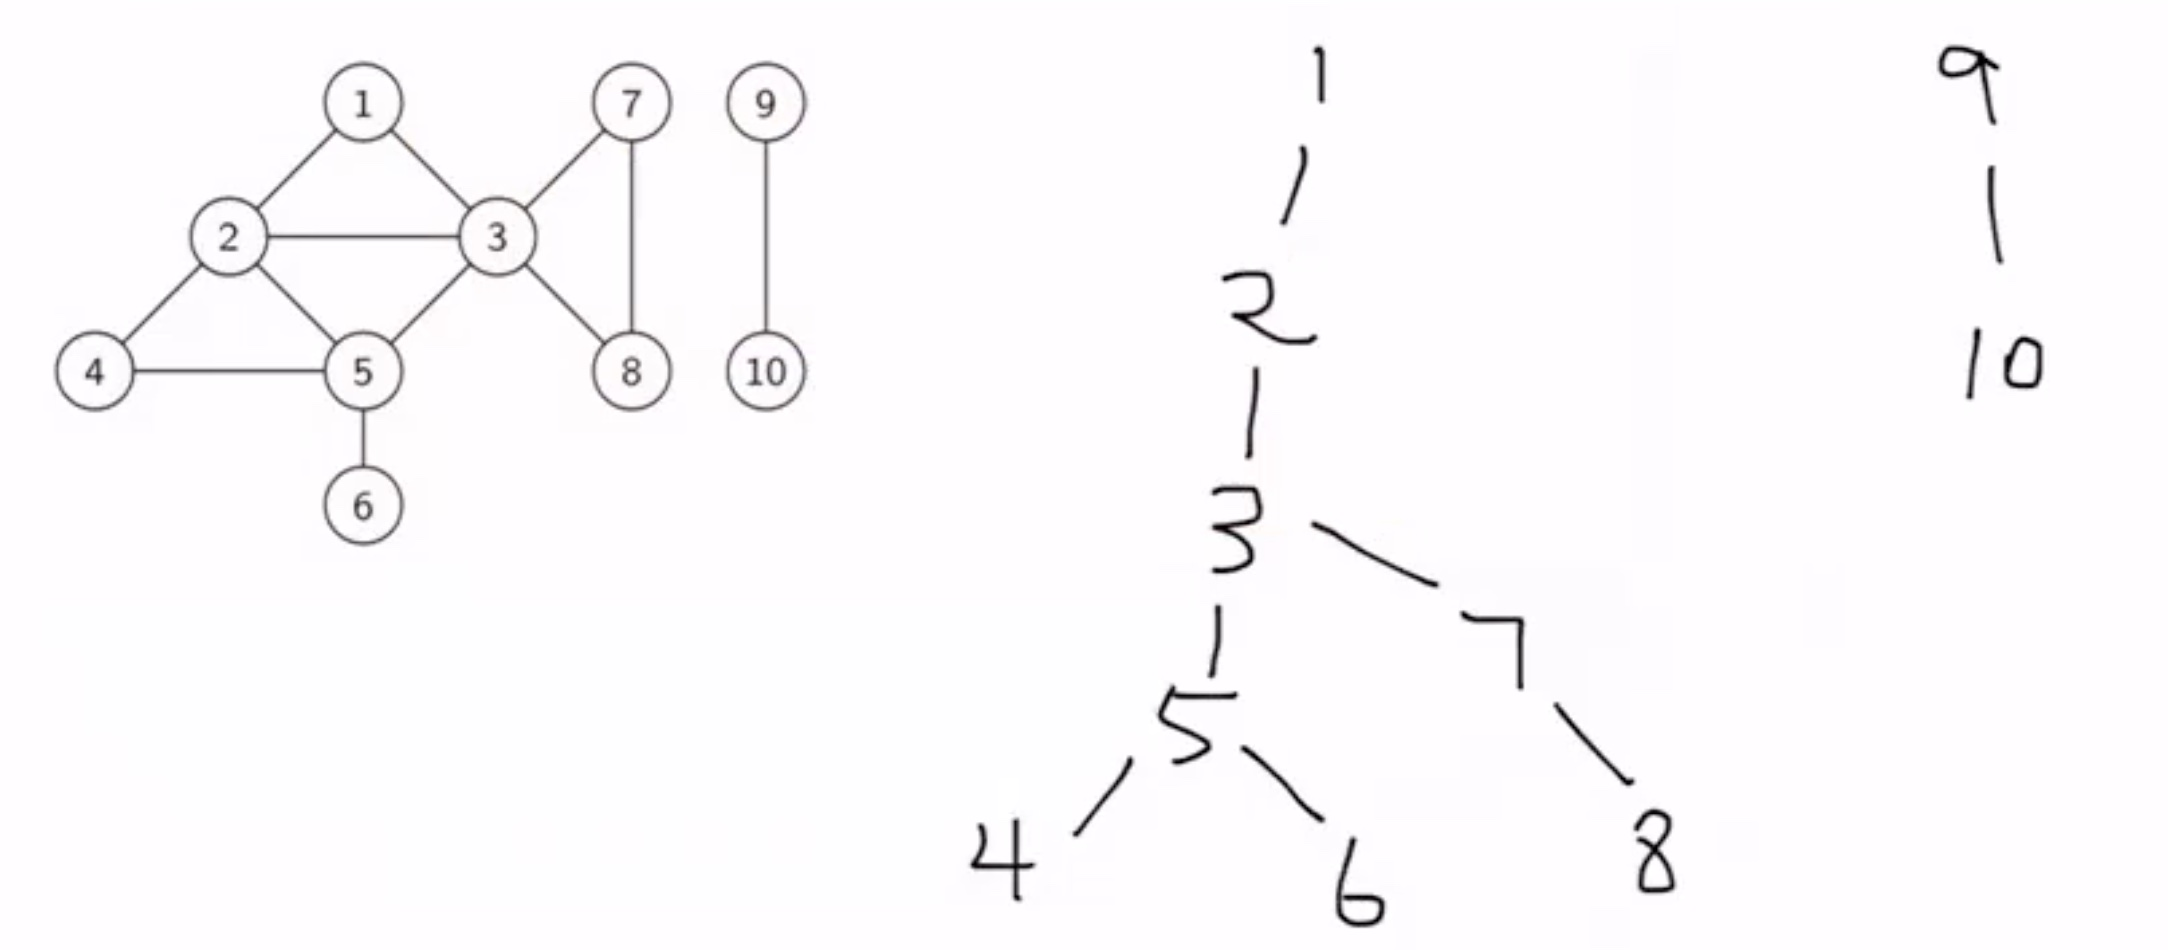
\includegraphics[width=0.725\textwidth]{lecture17/images/undirected-dfs-tree.jpg}
    \end{center}
    \item[] \lstinputlisting{lecture17/code/undirected-recursive-dfs.sudo}
    \item Edges are classified into two types: $uv \in E$ is a
    \begin{itemize}
        \item tree edge, it belongs to $T$
        \item non-tree edge, it does not belong to $T$
    \end{itemize}
    \item $T$ is a forest, and connected components of $T$ are the same as those of $G$.
    \item If $uv \in E$ is a non-tree edge, then either $u$ is an ancestor of $v$ or $v$ is an ancestor of $u$, in $T$.
    \item There are no cross edges.
\end{itemize}

\section{DFS with Visit Times}
\begin{itemize}
    \item We can keep track of when nodes are visited by including a timestamp.
    \item[] \lstinputlisting{lecture17/code/undirected-recursive-dfs-time.sudo}
    \begin{center}
        \item[] 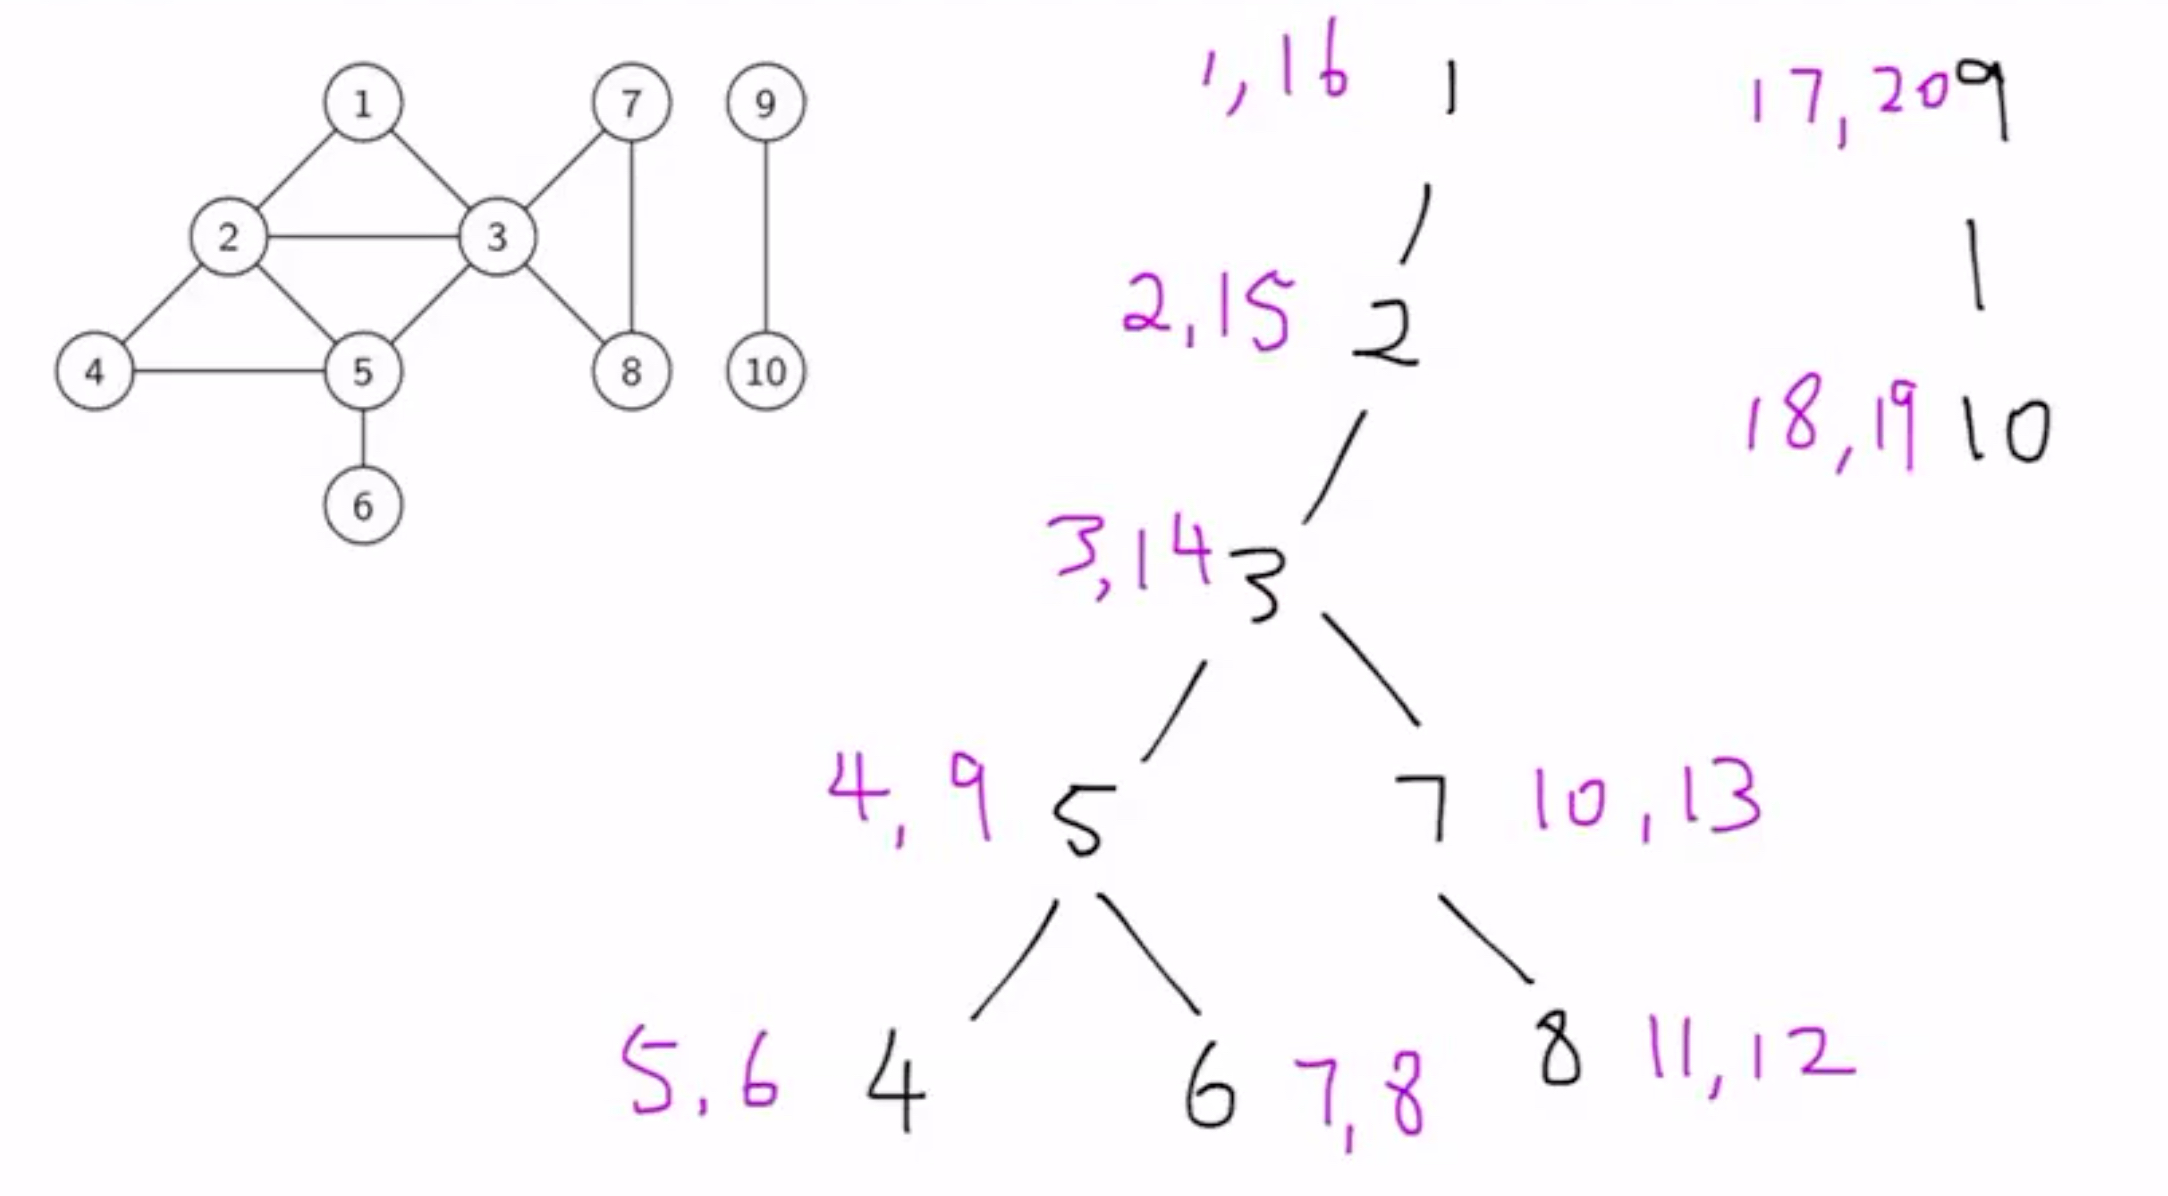
\includegraphics[width=0.75\textwidth]{lecture17/images/undirected-dfs-tree-time.jpg}
    \end{center}
    \item Node $u$ is active in the time interval $[ pre(u), post(u) ]$.
    \item For any two nodes $u$ and $v$, the two intervals $[pre(u), post(u)]$ and $[pre(v), post(v)]$ are disjoint or one is contained in the other.
    \begin{itemize}
        \item Assume without loss of generality that $pre(u) < pre(v)$. Then $v$ is visited after $u$.
        \item If \texttt{DFS($v$)} is invoked before \texttt{DFS(u)} finishes, then $post(v) < post(u)$.
        \item If \texttt{DFS($v$)} is invoked after \texttt{DFS(u)}, then $pre(v) > post(u)$.
    \end{itemize}
    \item $pre$ and $post$ numbers are useful in several applications of DFS.
\end{itemize}

\section{DFS in Directed Graphs}
\begin{itemize}
    \item[] \lstinputlisting{lecture17/code/directed-recursive-dfs-time.sudo}
    \item[] 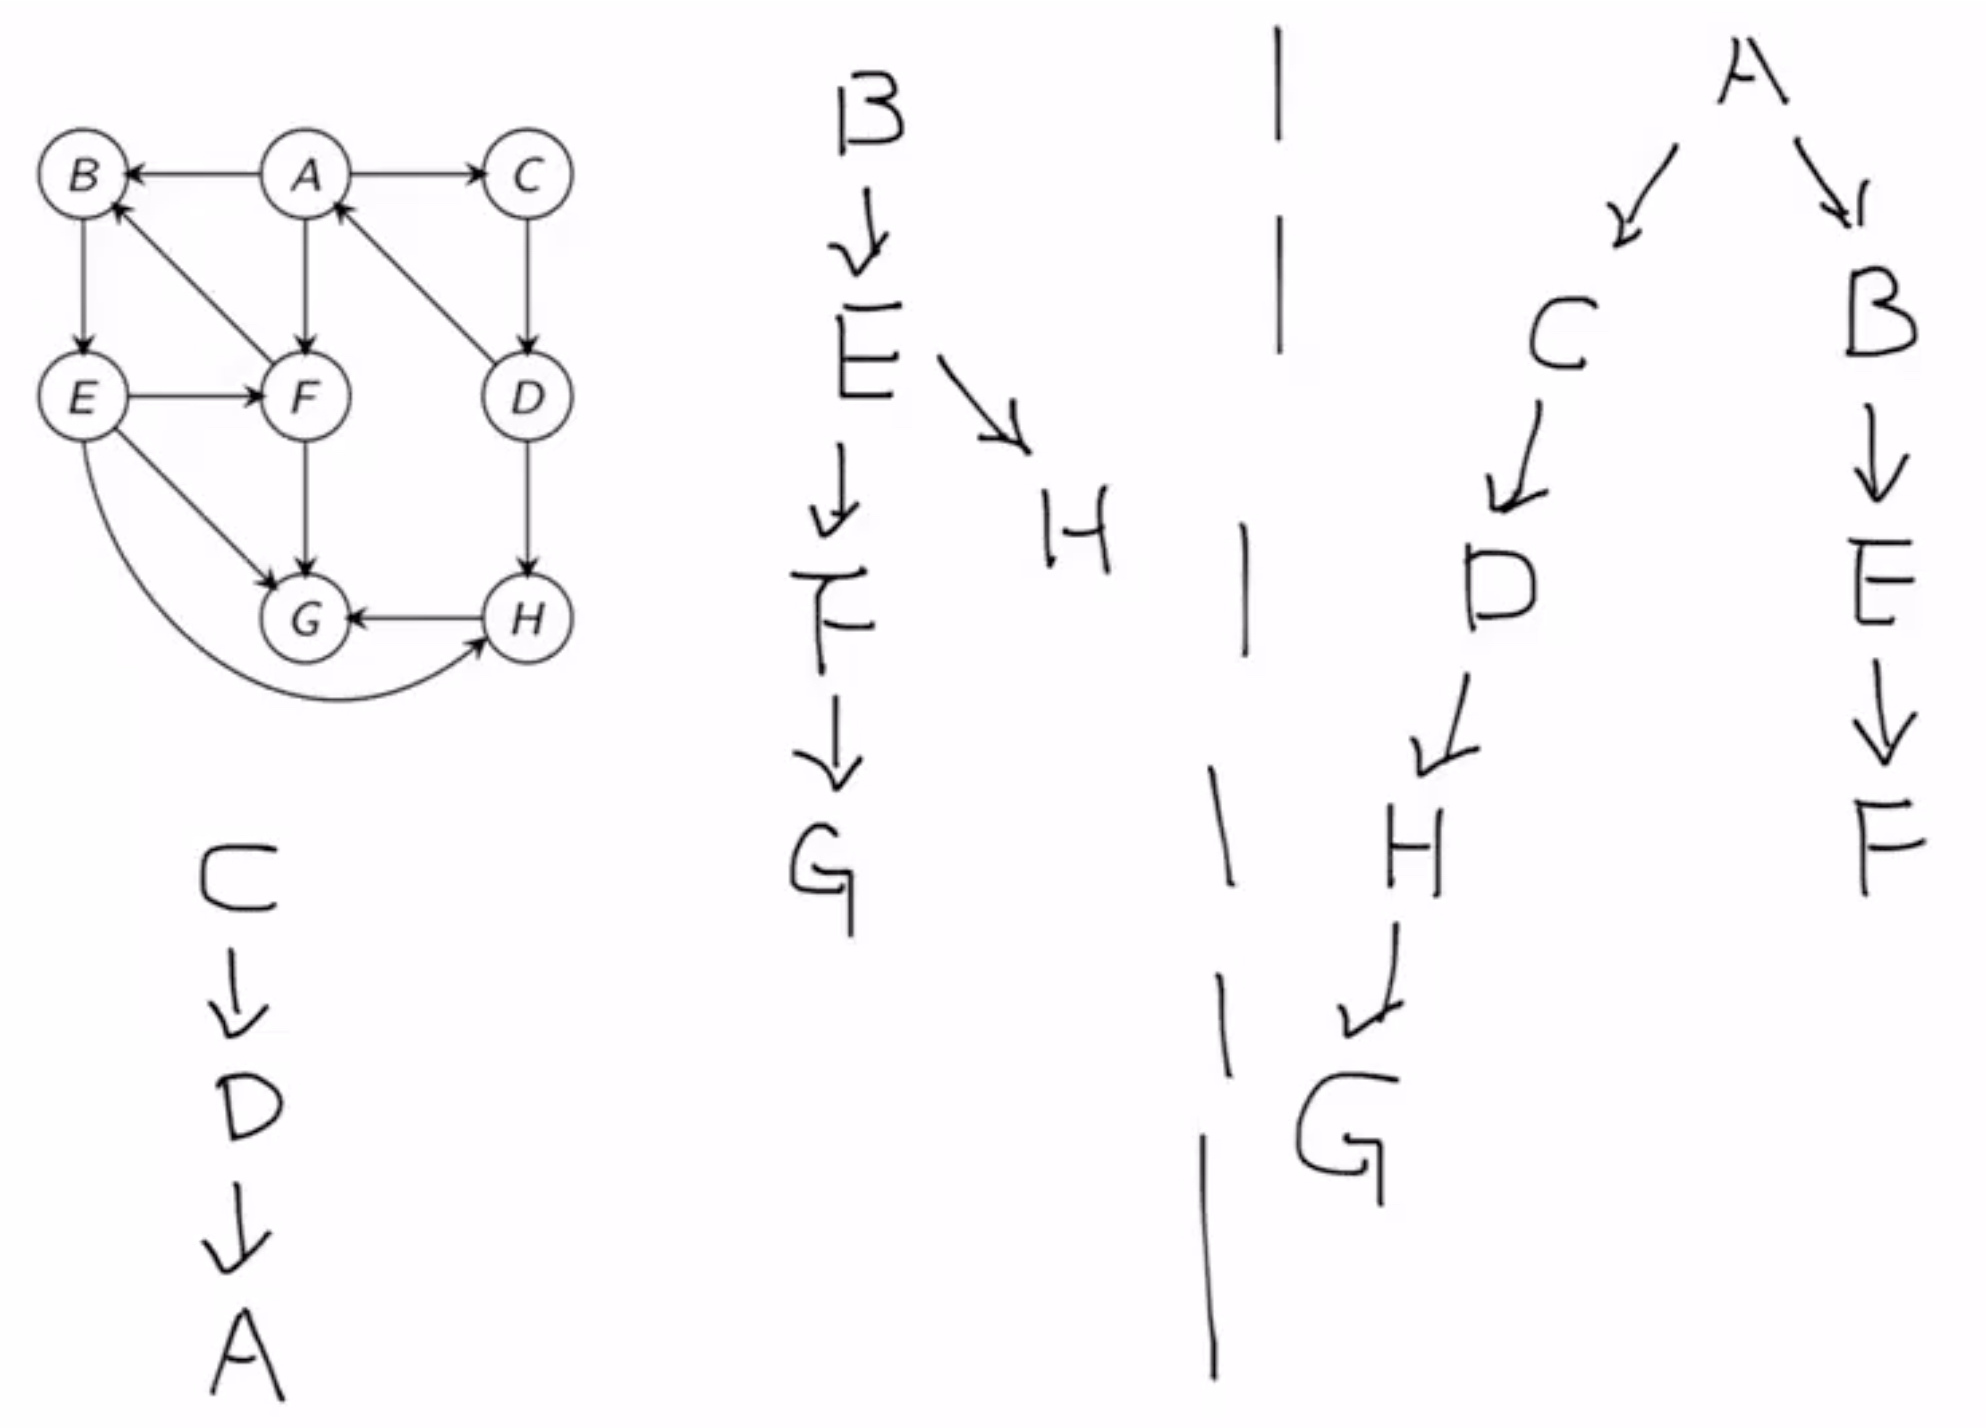
\includegraphics[width=0.8\textwidth]{lecture17/images/directed-dfs-tree-time.jpg}
    \item Generalizing ideas from undirected graphs:
    \begin{itemize}
        \item \texttt{DFS($G$)} takes $O(m + n)$ time.
        \item Edges added form a branching: a forest of out-trees. Output of \texttt{DFS($G$)} depends on the order in which vertices are considered.
        \item If $u$ is the first vertex considered by \texttt{DFS($G$)}, then \texttt{DFS($u$)} outputs a directed out-tree $T$ rooted at $u$, and a vertex $v$ is in $T$ if and only if $v \in rch(u)$.
        \item For any two vertices $x$ and $y$, the intervals $[pre(x), post(x)]$ and $[pre(y), post(y)]$ are either disjoint or one is contained in the other.
    \end{itemize}
    \item Edges of $G$ can be classified with respect to the DFS tree $T$ as
    \begin{itemize}
        \item Tree edges $(x, y)$ that belong to $T$:
        \item[] $pre(x) < pre(y) < post(y) < post(x)$
        \item Forward edges $(x, y)$ are non-tree edges:
        \item[] $pre(x) < pre(y) < post(y) < post(x)$
        \item Backward edges $(x, y)$ are non-tree edges:
        \item[] $pre(y) < pre(x) < post(x) < post(y)$
        \item Cross edges $(x, y)$ are non-tree edges:
        \item[] $pre(y) < post(y) < pre(x) < post(x)$
    \end{itemize}
    \item Note that what makes a backward edge special is $post(x) < post(y)$. Also note that both backward and cross edges have $pre(y) < pre(x)$.
    \begin{center}
        \item[] 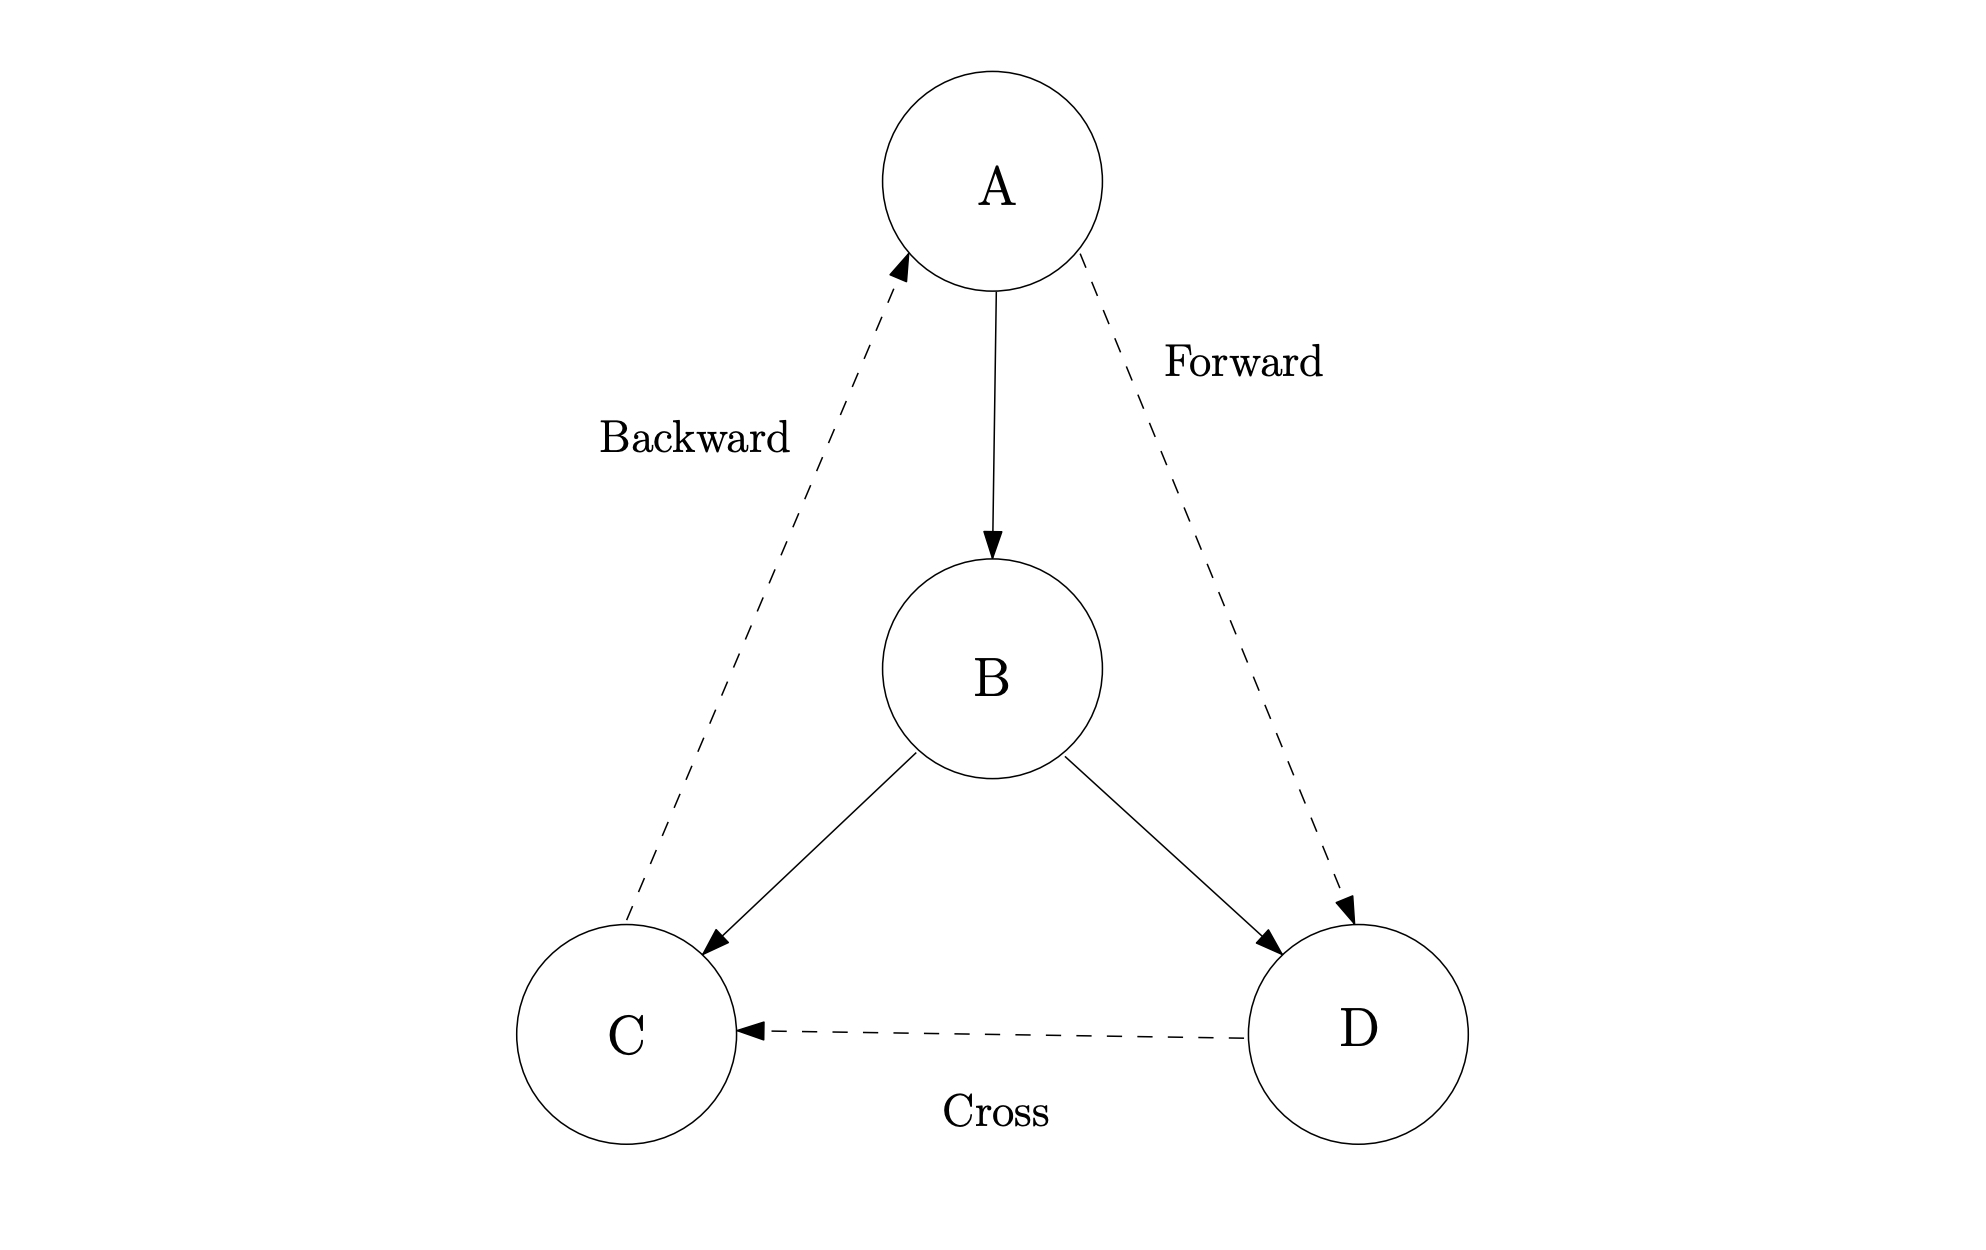
\includegraphics[width=0.6\textwidth]{lecture17/images/types-of edges.jpg}
    \end{center}
\end{itemize}

\subsection{Cycles in Graphs}
\begin{itemize}
    \item $G$ has a cycle if and only if there is a back edge in \texttt{DFS($G$)}.
    \begin{itemize}
        \item If: If $(u, v)$ is a back edge, then there is a cycle $C$ consisting of the path from $v$ to $u$ in the DFS search tree and the edge $(u, v)$.
        \item Only if: Suppose there is a cycle $C = v_1 \rightarrow v_2 \rightarrow ... \rightarrow v_k \rightarrow v_1$. Let $v_i$ be the first node in $C$ visited in DFS. All other nodes in $C$ are descendants of $v_i$ since they are reachable from $v_i$. Therefore, $(v_{i - 1}), v_i)$ (or $(v_k, v_1)$ if $i = 1$) is a back edge.
    \end{itemize}
    \item If $G$ is a DAG and $post(u) < post(v)$, then $(u, v)$ is not in $G$.
    \begin{itemize}
        \item Assume $post(u) < post(v)$ and $(u, v)$ is an edge in $G$. We can derive a contradiction. One of the two cases holds from DFS properties.
        \begin{enumerate}
            \item $[pre(u), post(u)]$ is contained in $[pre(v), post(v)]$: Implies that $u$ is explored during \texttt{DFS($v$)} and hence is a descendent of $v$. Edge $(u, v)$ implies a cycle in $G$ but $G$ is a DAG. Contradiction!
            \item $[pre(u), post(u)]$ is disjoint from $[pre(v), post(v)]$. This cannot happen since $v$ would be explored from $u$. Contradiction!
        \end{enumerate}
    \end{itemize}
\end{itemize}

\subsection{Using DFS with DAGs}
\begin{itemize}
    \item Given $G$, generate a topological sort if it is DAG, otherwise output a cycle $C$.
    \item Compute \texttt{DFS($G$)}
    \item If there is a back edge $e = (v, u)$, then $G$ is not a DAG. Output cycle $C$ formed by the path from $u$ to $v$ in $T$ plus edge $(v, u)$.
    \item Otherwise, output nodes in decreasing post visit order. There is no need to sort as \texttt{DFS($G$)} can output nodes in a correct order.
\end{itemize}

\section{DAGs, DFS, and SCC in Linear Time}

\subsection{Finding all SCCs of a Directed Graph}
\begin{itemize}
    \item Given a directed graph $G = (V, E)$, output all its strong connected components.
    \item A straightforward algorithm with running time $O(n(n + m))$:
    \item[] \lstinputlisting{lecture17/code/slow-scc.sudo}
\end{itemize}

\subsection{Graph of SCCs}
\begin{itemize}
    \item Let $S_1, S_2, ..., S_k$ be the strong connected components of $G$. The graph of SCCs is $G^{SCC}$.
    \begin{itemize}
        \item The vertices are $S_1, S_2, ..., S_k$.
        \item There is an edge $(S_i, S_j)$ if there is some $u \in S_i$ and $v \in S_j$ such that $(u, v)$ is an edge in $G$.
    \end{itemize}
    \item $G^{SCC}$ is created by collapsing every strong connected component to a single vertex.
    \item[] 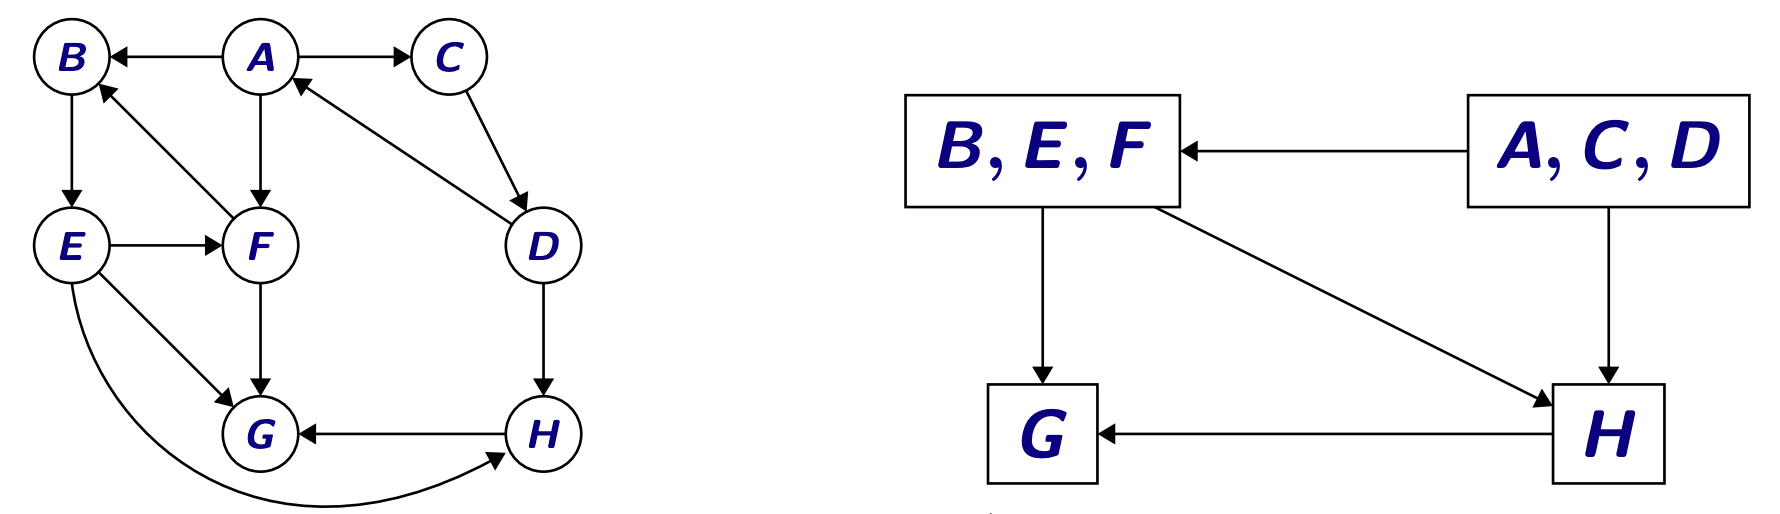
\includegraphics[width=\textwidth]{lecture17/images/meta-graph.jpg}
    \item For any graph $G$, the graph $G^{SCC}$ has no directed cycle. If $G^{SCC}$ has a cycle $S_1, S_2, ..., S_k$, then $S_1 \cup S_2, \cup ... \cup S_k$ should be in the same SCC in $G$.
\end{itemize}

\subsection{Linear-time Algorithm for SCCs}
\begin{itemize}
    \item We can generate a wishful thinking algorithm.
    \begin{itemize}
        \item Let $u$ be a vertex in a sink SCC of $G^{SCC}$.
        \item Do \texttt{DFS($u$)} to compute $SCC(u)$.
        \item Remove $SCC(u)$ and repeat.
    \end{itemize}
    \item Justification
    \begin{itemize}
        \item \texttt{DFS($u$)} only visits vertices (and edges) in $SCC(u)$ since there are no edges that come out of sink.
        \item \texttt{DFS($u$)} takes time proportional to size of $SCC(u)$, so the total time is $O(m + n)$.
    \end{itemize}
    \item The challenge of this algorithm if finding a vertex in a sink $SCC$ of $G^{SCC}$.
    \begin{itemize}
        \item We can try to obtain an implicit topological sort of $G^{SCC}$ without computing $G^{SCC}$.
        \item There is no easy way to find a node in a sink SCC, but there is a way to find a node in a source SCC. Then, we can find a node in the source SCC of the reversal of $G^{SCC}$.
        \item For any graph $G$, the graph of SCCs of $G^{rev}$ is the same as the reversal of $G^{SCC}$. The SCCs of $G^{rev}$ are the same as those of $G$.
    \end{itemize}
    \item If $C$ and $C'$ are SCCs, and there is an edge from a node in $C$ to a node in $C'$, then the highest post number in $C$ is bigger than the highest post number in $C'$. Consider two cases:
    \begin{enumerate}
        \item DFS visits $C$ first: All vertices will be traversed. The first node visited in $C$ will have the highest post number.
        \item DFS visits $C'$ first: DFS will stop after visiting all nodes in $C'$, but before seeing any of $C$.
    \end{enumerate}
    \item The node that receives the highest post number in DFS must lie in a source SCC. Thus, the SCCs are topologically sorted by arranging them in decreasing order of their highest post number. 
    \item[] \lstinputlisting{lecture17/code/linear-scc.sudo}
\end{itemize}

\subsection{Linear-time Algorithm for SCCs Example}
\begin{itemize}
    \item[] 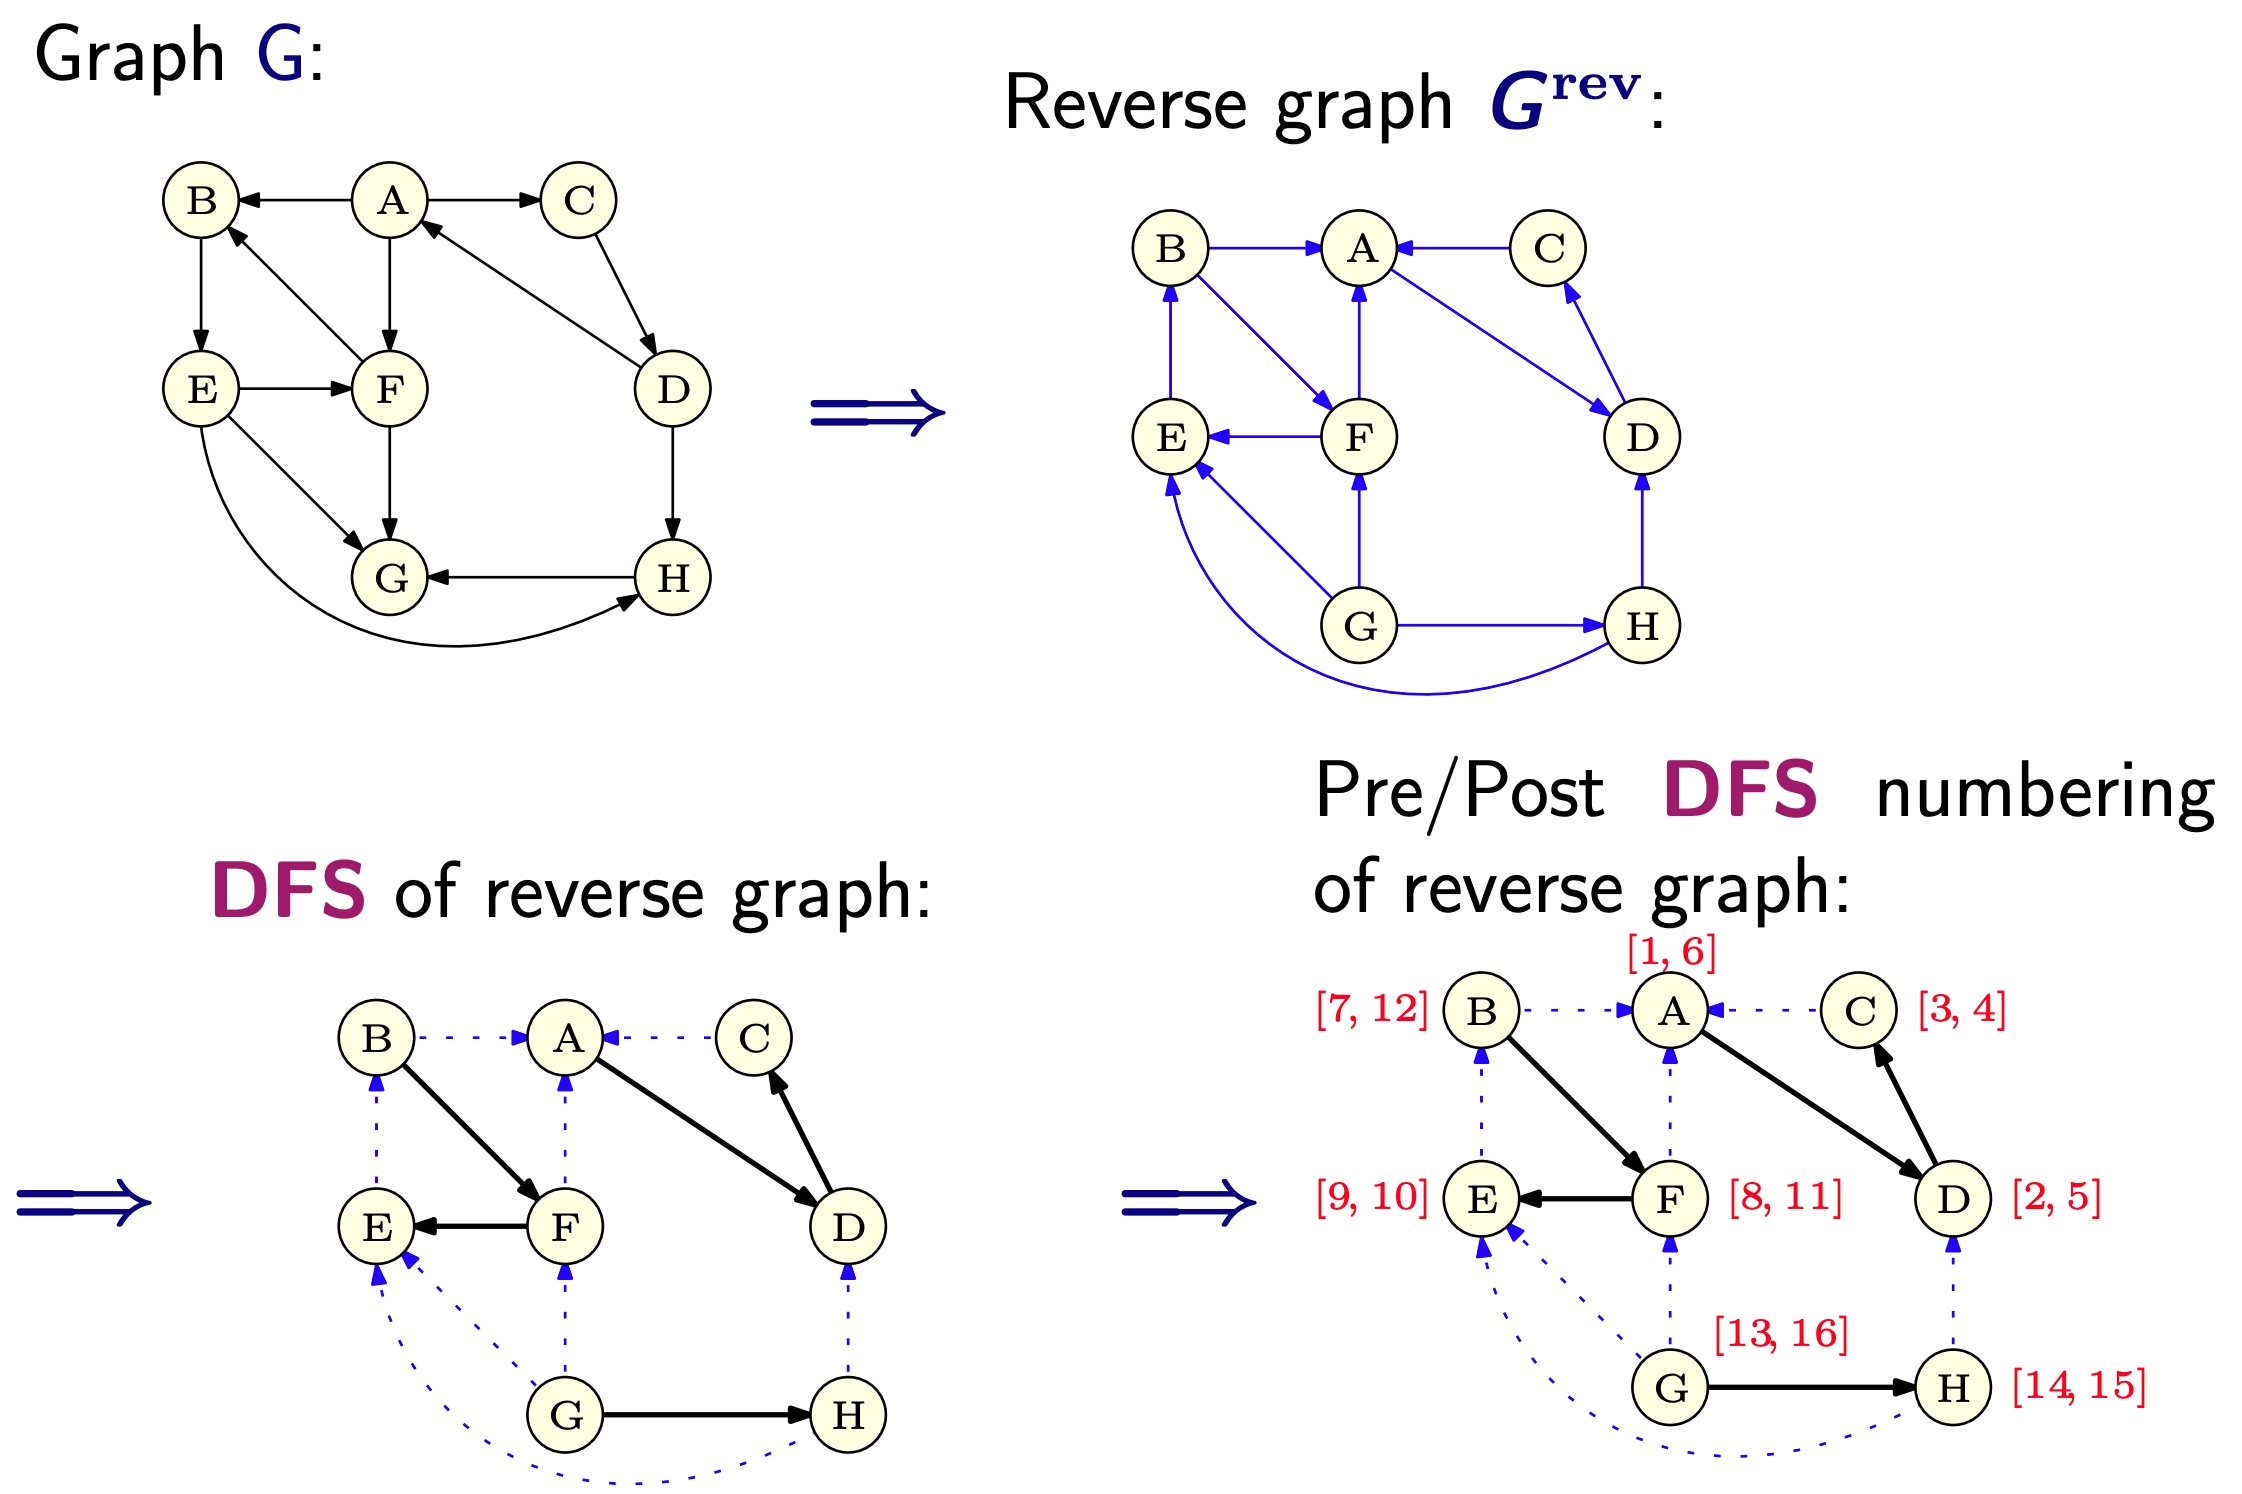
\includegraphics[width=\textwidth]{lecture17/images/linear-scc-algorithm-visualization.jpg}
    \item[] 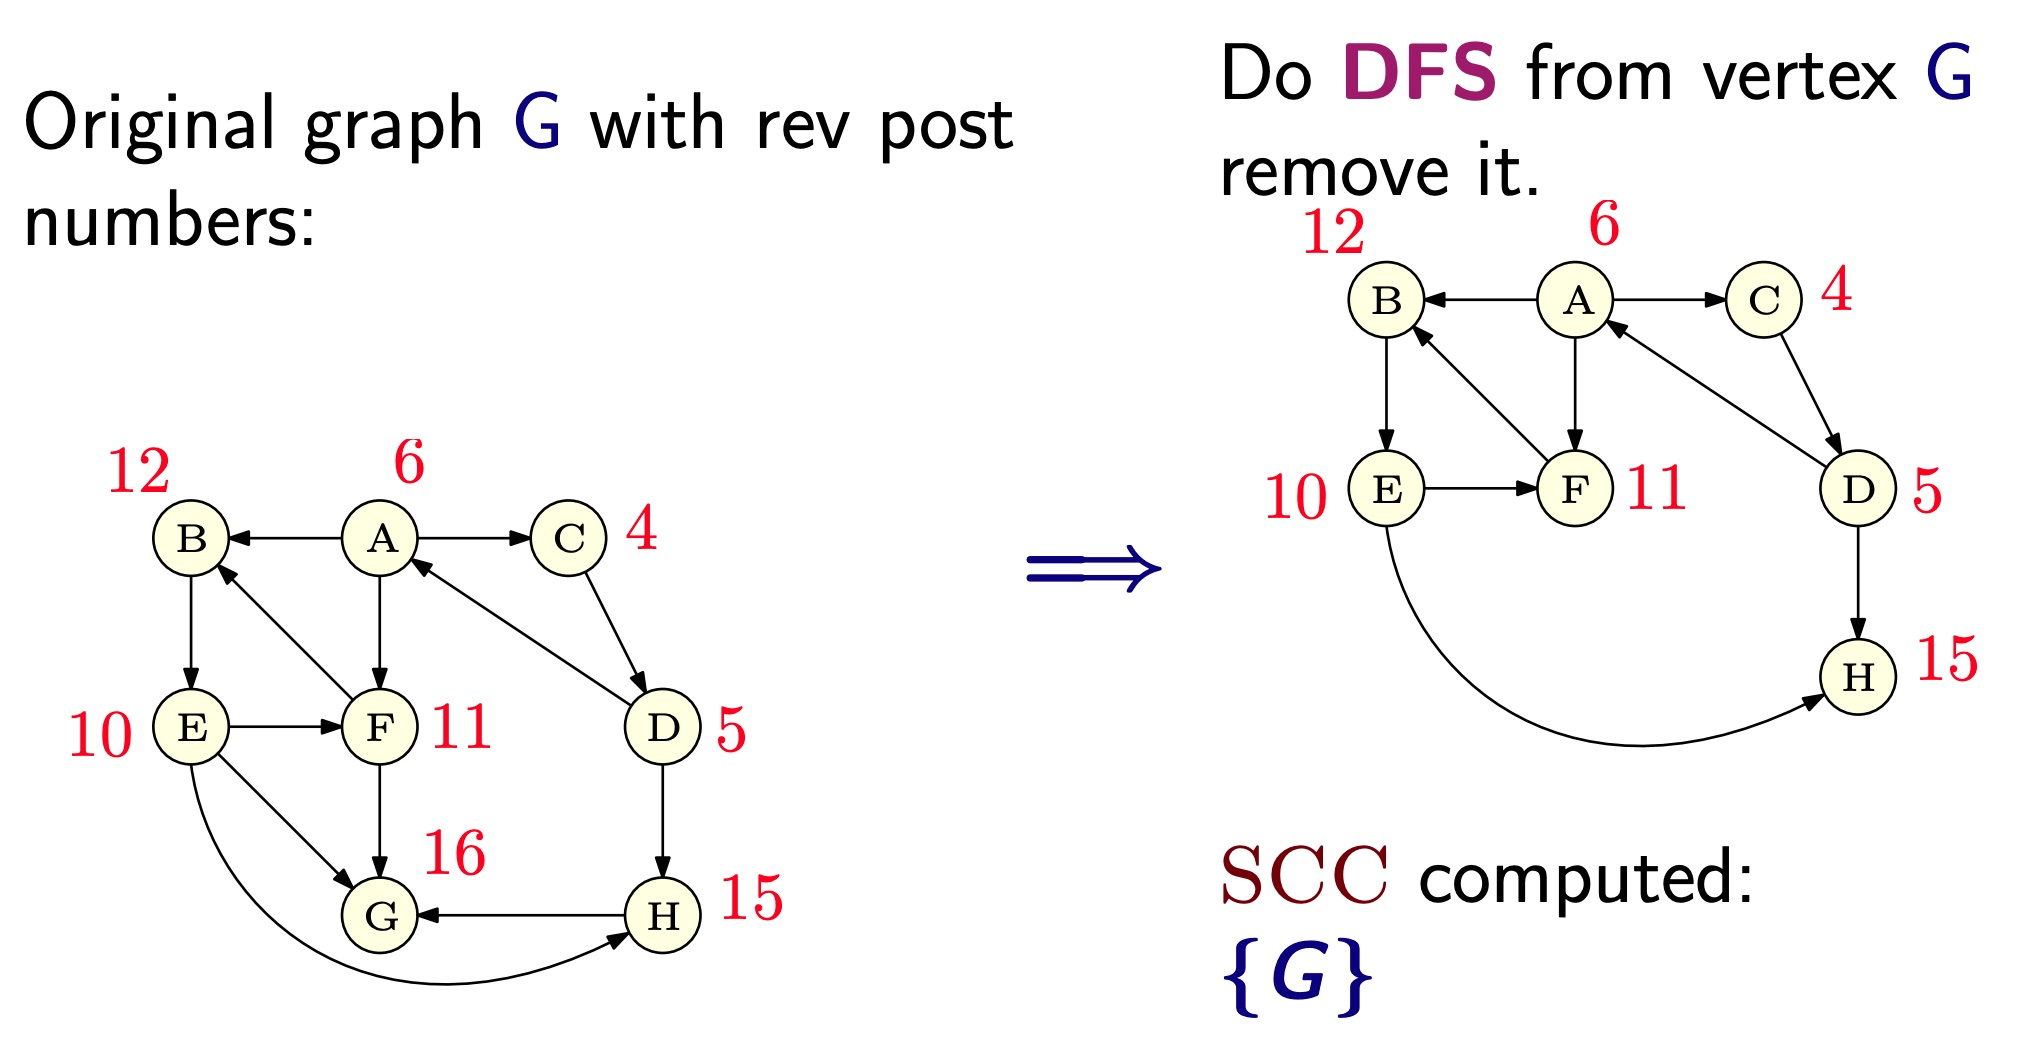
\includegraphics[width=\textwidth]{lecture17/images/linear-scc-algorithm-visualization-2.jpg}
    \item We repeat this process till we reach the computed SCC of $\{ G \}, \{ H \}, \{ F, B, E \}, \{ A, C, D \}$.
    \item We can use this algorithm as a template for solving problems on directed graphs.
    \begin{itemize}
        \item Is the problem solvable when $G$ is strongly connected?
        \item Is the problem solvable when $G$ is a DAG?
        \item If the above two are feasible, then is the problem solvable in a general directed graph $G$ by considering the meta graph $G^{SCC}$?
    \end{itemize}
\end{itemize}

\subsection{Take Away Points}
\begin{itemize}
    \item Given a directed graph $G$, its SCCs and the associated acyclic meta-graph $G^{SCC}$ give a structural decomposition of $G$ that should be kept in mind.
    \item There is a DFS based linear time algorithm to compute all the SCCs and the meta-graph. Properties of DFS are crucial for the algorithm.
    \item DAGs arise in many applications, and topological sort is a key property in algorithm design. Linear time algorithms can compute a topological sort. There can be many possible orderings, so they are not unique.
\end{itemize}
